\section{Penelitian dan Riset Terkait}
\label{sec:riset-terkait}
Berikut adalah beberapa penelitian dan riset yang pernah dilakukan sebelumnya dan berhubungan dengan tugas akhir ini.

\subsection{LEONORE, \textit{Large-Scale Provisioning of
    Resource Constrained
    IoT Deployments}}
Riset dilakukan oleh Michael Vogler, Johannes M. Schleicher, Christian Inzinger, Stefan Nastic, Sanjin Sehic and Schahram Dustdar dari Vienna University of Technology. Riset ini menjelaskan mengenai cara pembuatan sebuah infrastruktur untuk melakukan \textit{provisioning} perangkat \textit{IoT} dalam skala besar.

\subsection{China Electronic Toll Colleciton}
China memiliki masyarakat yang sangat banyak dan setiap masyarakat memiliki sekurang kurangnya satu kendaraan. Seiring bertambah nya masyarakat di China, maka jalanan yang ada di China akan semakin penuh dengan kendaraan yang akan menghasilkan kemacetan terutama pada tol bagian pembayaran. Untuk mengatasi masalah ini China menggunakan \textit{Electronic Toll Colleciton (ETC)} yang di integrasikan dengan setiap kendaraan untuk mempercepat proses ini \parencite{penelitianterkait1}.

China menggunakan KubeEdge untuk melakukan proses \textit{deployment} \textit{ETC} untuk 100,000 \textit{nodes} dengan total 500,000 aplikasi yang diluncurkan menggunakan KubeEdge tersebar untuk 29 dari 34 provinsi. Proses \textit{deployment} dilakukan secara otomatis dengan membuat sistem \textit{workflow engine} pada kubernetes sehingga proses \textit{deployment} dapat dilakukan dengan cepat dan mudah. Dengan menggunakan metode ini sistem pembayaran tol di China menjadi 10x lebih cepat dari sebelumnya \parencite{penelitianterkait1}.

\begin{figure}[ht]
  \centering
  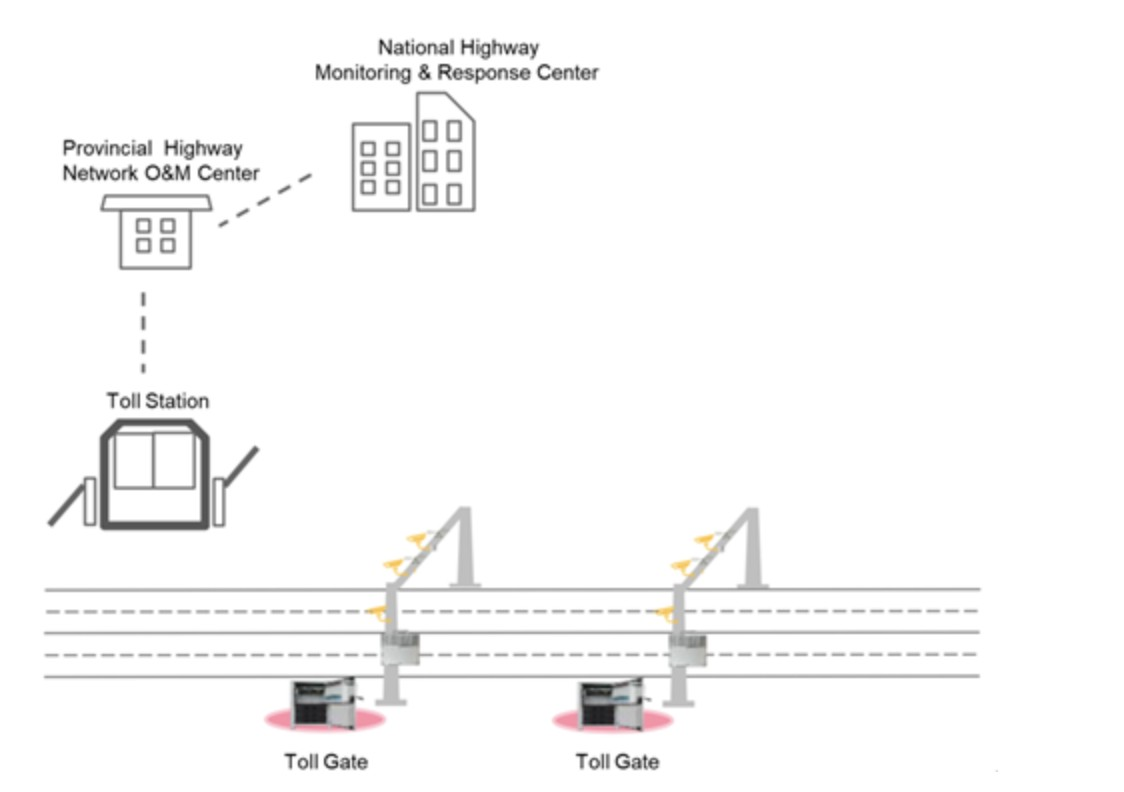
\includegraphics[width=0.8\textwidth]{resources/chapter-2/china-highways.jpg}
  \caption{Implementasi Sistem \textit{ETC} di China \parencite{penelitianterkait1}}
  \label{fig:china-highways}
\end{figure}

\begin{figure}[ht]
  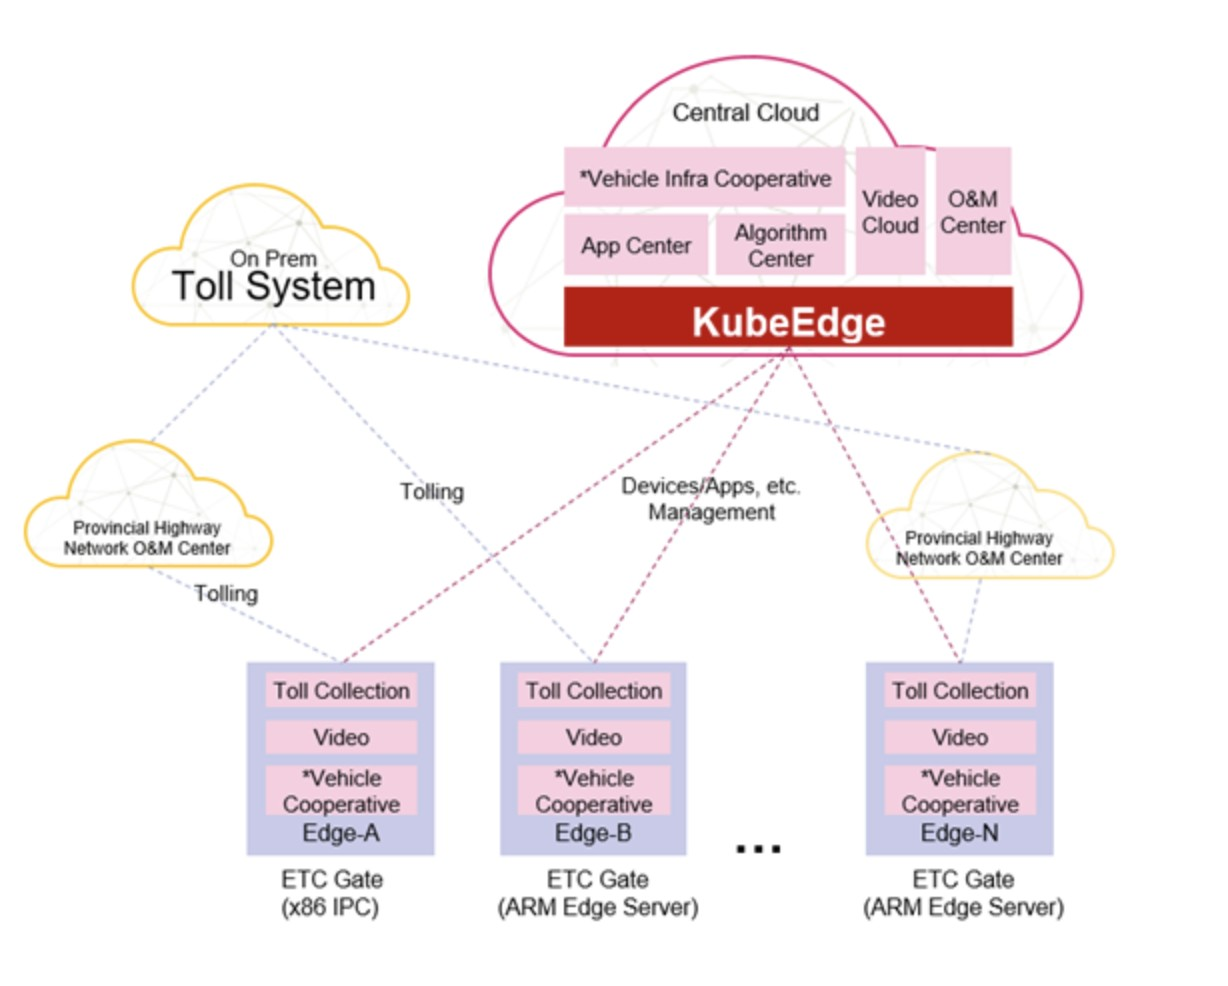
\includegraphics[width=0.8\textwidth]{resources/chapter-2/arsitektur-china-highways.jpg}
  \caption{Arsitektur Sistem \textit{ETC} di China \parencite{penelitianterkait1}}
  \label{fig:architecture-china-highways}
\end{figure}
\subsection{A Model for the Remote Deployment, Update, and Safe Recovery for Commercial Sensor-Based IoT Systems}
Penelitian ini menggali tantangan-tantangan khusus terkait infrastruktur yang didedikasikan untuk penyebaran dan manajemen aplikasi secara jarak jauh. Penelitian ini membahas tantangan-tantangan manajemen terkait sistem sensor IoT dan mengusulkan sebuah cara serta metodologi untuk mengatasi hal tersebut.

Penelitian ini mengimplementasikan solusi sebagai sistem infrastruktur perangkat lunak untuk produk IoT bisnis yang lengkap. Penelitian ini melakukan \textit{deployment} pada 100 perangkat penjual minuman yang tersebar di tiga lokasi. Setiap perangkat bergantung pada sensor yang memantau statusnya dan pada \textit{gateway} yang mengendalikan perilakunya. Arsitektur sistem dapat dilihat pada gambar \ref{fig:architecture-remote-deployments}.

\begin{figure}[ht]
  \centering
  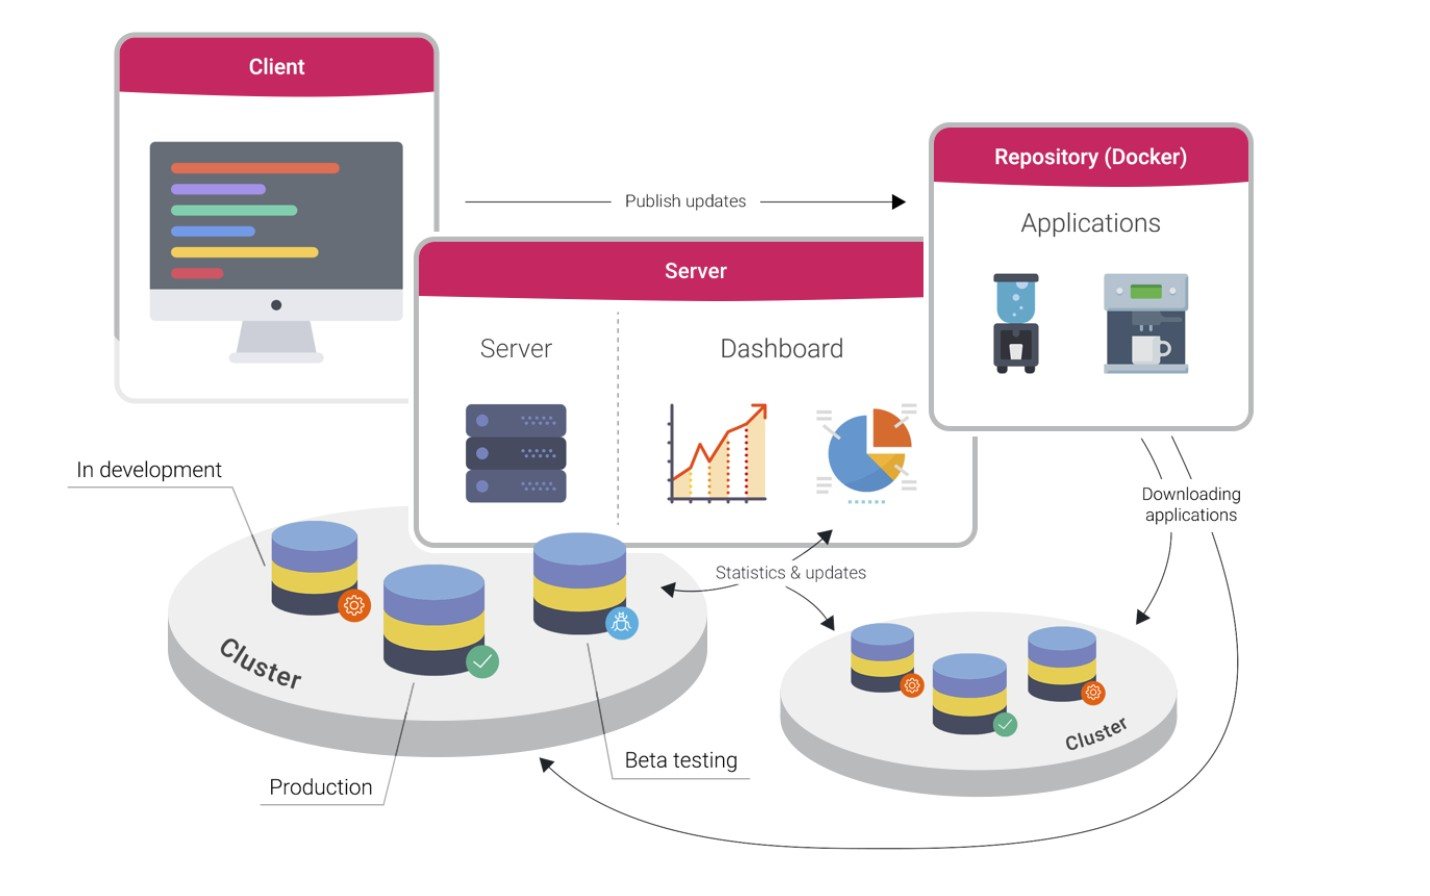
\includegraphics[width=0.8\textwidth]{resources/chapter-2/arsitektur-remote-deployment.jpg}
  \caption{Arsitektur Remote \textit{Deployment} \parencite{RemoteDeployment}}
  \label{fig:architecture-remote-deployments}
\end{figure}

Selama penelitian ini berlangsung, penelitian ini berhasil menerima 133 \textit{update} pada perangkat IoT. 80\% perangkat beroperasi tanpa gangguan selama 250 hari. Sedangkan, 20\% mengalami kegagalan akibat faktor eksternal. Dari 80\% tersebut, 30\% mengalami kegagalan pembaruan sementara akibat kapabilitas perangkat yang berkurang \parencite{RemoteDeployment}.

Solusi yang dibuat penelitian ini mengandalkan keamanan serta \textit{failsafe} yang dapat melakukan \textit{remote deployment} dengan baik serta aman sehingga dapat mendeteksi kegagalan yang terjadi pada perangkat dan melakukan \textit{recovery} dengan cepat. Berikut merupakan beberapa cara untuk melakukan \textit{remote deployment} atau seringkali disebut sebagai OTA \textit{(Over the air)}.

\begin{figure}[ht]
  \centering
  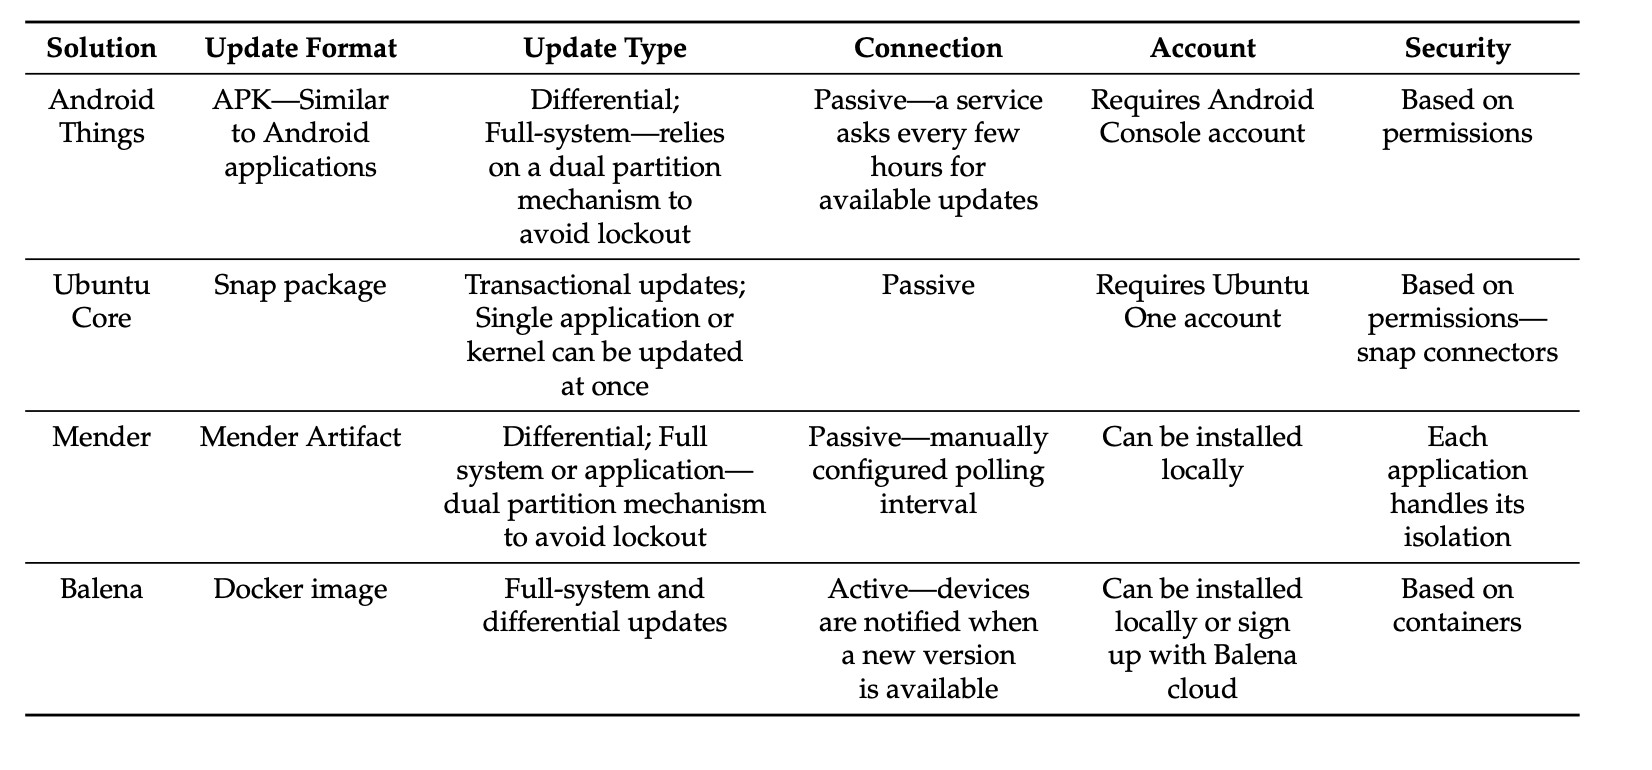
\includegraphics[width=0.8\textwidth]{resources/chapter-2/perbandingan-remote-deployment.jpg}
  \caption{Perbandingan Tata Cara \textit{Remote Deployment} \parencite{RemoteDeployment}}
  \label{fig:comparison-remote-deployments}
\end{figure}

Dapat dilihat dari gambar \ref{fig:comparison-remote-deployments} bahwa terdapat berbagai solusi untuk berbagai tipe \textit{remote deployment}. Pada kasus ini, dapat dibuat suatu cara yang mengadopsi \textit{update type} serta koneksi dari keempat tipe tersebut. Perangkat melakukan \textit{polling} kepada \textit{server} untuk mengecek apakah terdapat versi terbaru atau tidak. Selain itu, dari sisi \textit{Server} juga dapat membuat suatu notifikasi yang dapat diterima oleh perangkat jika terdapat \textit{update} baru yang siap digunakan.

% \subsection{Penelitian Lainnya}

% Adapun \textit{autoscaler} yang sudah dikembangkan dan dibahas di banyak penelitian lain. Pendekatan dan metode yang digunakan sangat variatif. Gambaran umum mengenai penelitian lain yang berhubungan dengan \textit{autoscaler} menggunakan model prediksi, \textit{threshold} atau \textit{rule based} maupun \textit{machine learning} bisa dilihat pada tabel \ref{tab:overview-autoscaler}.

% \begin{longtable}{|p{2in}|c|p{1in}|c|p{0.8in}|}

%     \caption{Tabel Penelitian Lain terkait Pengembangan Metode \textit{Autoscaling}} \label{tab:overview-autoscaler} \\

%     \hline
%     \rowcolor{gray!30}\multicolumn{1}{|c|}{\textbf{Paper}} & \textbf{Virtualisasi} & \multicolumn{1}{|c|}{\textbf{Metrik}} & \textbf{Pendekatan} & \multicolumn{1}{|c|}{\textbf{Metode}} \\
%     \hline
%     \endfirsthead
%     %
%     \endhead
%     %
%     \textit{Intelligent Workload Factoring for a Hybrid Cloud Computing Model}, \parencite{zhang} & VM & \textit{Request Rate} & Reaktif & ARIMA \tabularnewline

%     \textit{Autonomic Vertical Elasticity of Docker Containers with Elasticdocker}, \parencite{al2017autonomic} & \textit{Container} & Prosesor, Memori & Reaktif & \textit{Rule-based} \tabularnewline

%     \textit{Horizontal Pod Autoscaler}, \parencite{hpa2} & \textit{Container} & Prosesor & Reaktif & \textit{Rule-based} \tabularnewline

%     \textit{A Novel Resource Prediction and Provisioning Scheme in Cloud Data Center}, \parencite{rpps} & \textit{Container} & Prosesor & Proaktif & ARMA \tabularnewline

%     \textit{Workload Prediction Using ARIMA Model and Its Impact on Cloud Applications QoS}, \parencite{workloadprediction} & VM & \textit{Request Rate} & Proaktif & ARIMA \tabularnewline

%     \textit{Resource Elasticity Controller for Docker-based Web Applications}, \parencite{resourceelasticity} & \textit{Container} & \textit{Request Rate} & Proaktif & ARIMA \tabularnewline

%     \textit{Combining Time Series Prediction Models using Genetic Algorithm to Autoscaling Web Applications Hosted in the Cloud Infrastructure}, \parencite{tspwithga} & - & \textit{Request Rate} & Proaktif & \textit{Genetic Algorithm} \tabularnewline

%     \textit{Predicting Cloud Resource Provisioning using Machine Learning Techniques}, \parencite{predictcloudrsrc} & - & \textit{Task Length} & Proaktif & \textit{Artificial Neural Network} \tabularnewline

%     \textit{Auto-scaling Microservices on IaaS under SLA with Cost-Effective Framework}, \parencite{asmicrocosteff} & VM & \textit{Request Rate} & Proaktif & \textit{Artificial Neural Network}, \textit{Recurrent Neural Network} \tabularnewline

%     \textit{Machine Learning-based Auto-scaling for Containerized Applications}, \parencite{mlbasconapps} & \textit{Container} & \textit{Request Rate} & Proaktif & LSTM \tabularnewline

%     \textit{Adaptive Horizontal Scaling of Microservices using Bi-LSTM}, \parencite{adaptivehsmicro} & \textit{Container} & Prosesor, Memori & Gabungan & Bi-LSTM \tabularnewline

%     \hline
% \end{longtable}